\documentclass[tikz,border=2pt]{standalone}
\usepackage[T1]{fontenc}\usepackage{helvet}\usepackage{amsmath}
% shared TikZ styles for the three block diagrams (editable sources)
\usetikzlibrary{arrows.meta,positioning,fit,calc,backgrounds,shapes.geometric}
\definecolor{learn}{HTML}{6250D6}   % learned components
\definecolor{numer}{HTML}{2A78D6}   % numerical methods (Kalman lineage)
\definecolor{numerh}{HTML}{EB6834}  % numerical methods (Khalil lineage)
\definecolor{check}{HTML}{1D6B43}   % deterministic checks
\definecolor{ink}{HTML}{1B2430}
\definecolor{mut}{HTML}{5D6B7A}
\tikzset{
  every node/.style={font=\sffamily\scriptsize,text=ink,execute at begin node={\hyphenpenalty=10000 \exhyphenpenalty=10000 }},
  box/.style={draw=mut,rounded corners=1.5pt,line width=0.5pt,align=center,inner sep=3.5pt,fill=white,minimum height=6.5mm},
  learned/.style={box,draw=learn,dashed,line width=0.8pt,fill=learn!7},
  numeric/.style={box,draw=numer,line width=0.8pt,fill=numer!7},
  numerich/.style={box,draw=numerh,line width=0.8pt,fill=numerh!8},
  checkb/.style={box,draw=check,line width=0.8pt,double,double distance=0.6pt,fill=check!6},
  user/.style={box,fill=black!5},
  arr/.style={-{Stealth[length=4pt,width=3.4pt]},line width=0.5pt,draw=ink},
  darr/.style={arr,dashed},
  lab/.style={font=\sffamily\fontsize{6}{7}\selectfont,text=mut,align=center},
  onl/.style={lab,fill=white,inner sep=1.5pt},
  group/.style={draw=mut,dotted,line width=0.6pt,rounded corners=3pt,inner sep=5pt},
}

\tikzset{every node/.append style={font=\sffamily\footnotesize}, lab/.style={font=\sffamily\fontsize{7}{8}\selectfont,text=mut,align=center},
         onl/.style={lab,fill=white,inner sep=1.5pt}, sig/.style={font=\sffamily\fontsize{7.5}{8.5}\selectfont,text=ink,fill=white,inner sep=1pt}}
\begin{document}
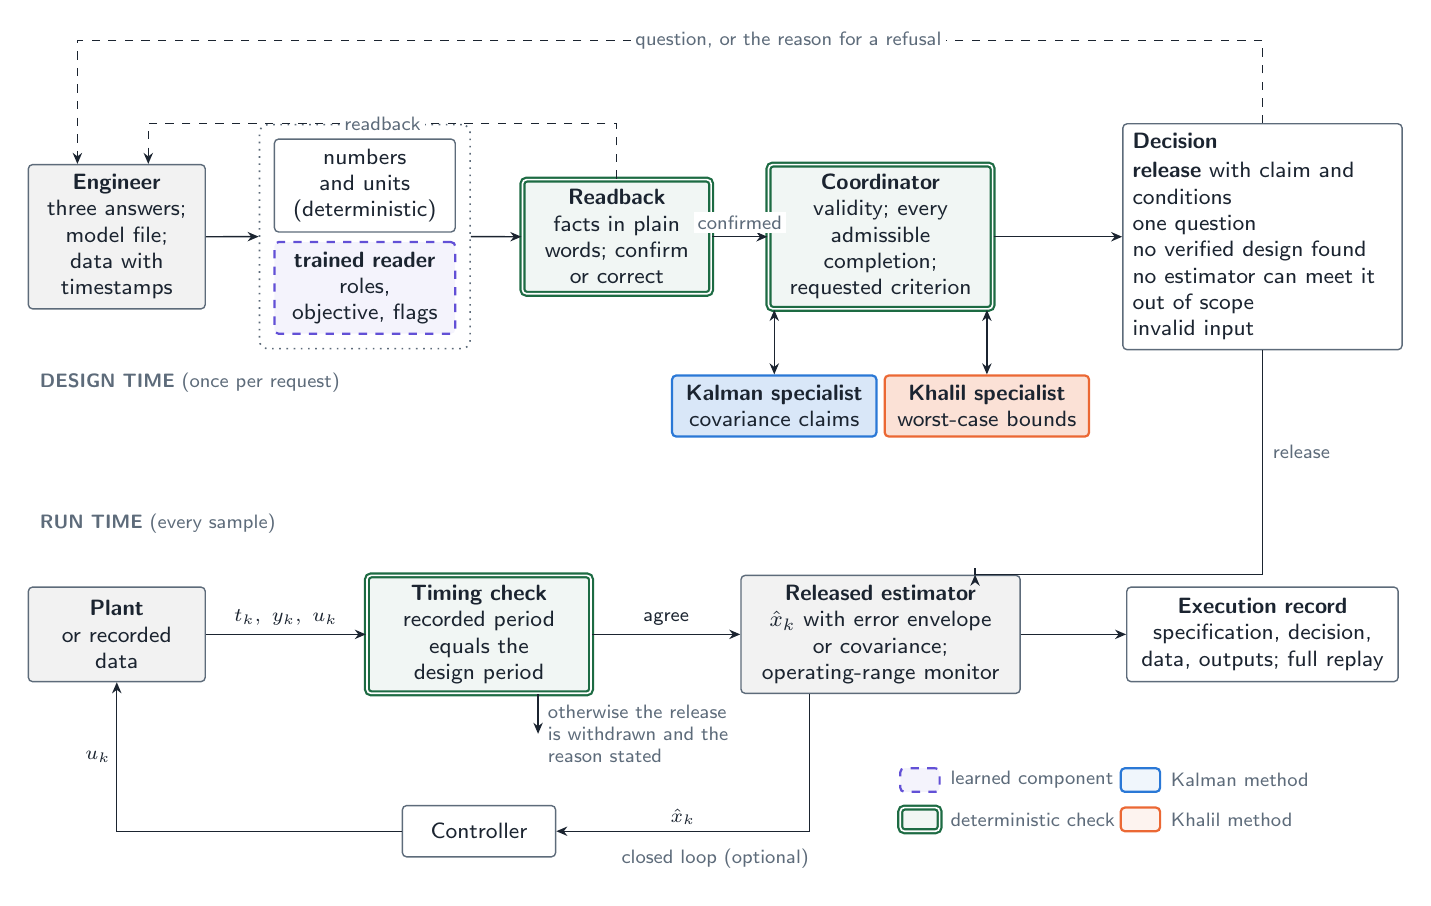
\begin{tikzpicture}[x=1cm,y=1cm]
% ================= design time: request -> decision =================
\node[lab,anchor=west] at (-1.1,3.75) {\textbf{DESIGN TIME} (once per request)};
\node[user,text width=2.0cm,minimum height=1.45cm] (U) at (0,5.6) {\textbf{Engineer}\\ three answers; model file; data with timestamps};
\node[box,text width=2.05cm] (Q) at (3.15,6.25) {numbers and units (deterministic)};
\node[learned,text width=2.05cm] (R) at (3.15,4.95) {\textbf{trained reader}\\ roles, objective, flags};
\node[checkb,text width=2.15cm,minimum height=1.45cm] (B) at (6.35,5.6) {\textbf{Readback}\\ facts in plain words; confirm or correct};
\node[checkb,text width=2.6cm,minimum height=1.45cm] (C) at (9.7,5.6) {\textbf{Coordinator}\\ validity; every admissible completion; requested criterion};
\node[numeric,fill=numer!18,text width=2.35cm] (K) at (8.35,3.45) {\textbf{Kalman specialist}\\ covariance claims};
\node[numerich,fill=numerh!20,text width=2.35cm] (H) at (11.05,3.45) {\textbf{Khalil specialist}\\ worst-case bounds};
\node[box,text width=3.3cm,align=left] (D) at (14.55,5.6) {\textbf{Decision}\\[1pt] \textbf{release} with claim and conditions\\ one question\\ no verified design found\\ no estimator can meet it\\ out of scope\\ invalid input};
\begin{scope}[on background layer]
\node[group,fit=(Q)(R)] (I) {};
\end{scope}
\draw[arr] (U.east) -- (I.west);
\draw[arr] (I.east) -- (B.west);
\draw[arr] (B.east) -- node[onl,above=1pt]{confirmed} (C.west);
\draw[arr,{Stealth[length=4pt,width=3.4pt]}-{Stealth[length=4pt,width=3.4pt]}] (K.north) -- (K.north |- C.south);
\draw[arr,{Stealth[length=4pt,width=3.4pt]}-{Stealth[length=4pt,width=3.4pt]}] (H.north) -- (H.north |- C.south);
\draw[arr] (C.east) -- (D.west);
\draw[darr] (B.north) -- ++(0,0.7) -| node[onl,pos=0.25]{readback} ($(U.north)+(0.4,0)$);
\draw[darr] (D.north) -- ++(0,1.05) -| node[onl,pos=0.2]{question, or the reason for a refusal} ($(U.north)+(-0.5,0)$);
% ================= run time: signals =================
\node[lab,anchor=west] at (-1.1,1.95) {\textbf{RUN TIME} (every sample)};
\node[box,fill=black!5,text width=2.0cm,minimum height=1.2cm] (P) at (0,0.55) {\textbf{Plant}\\ or recorded data};
\node[checkb,text width=2.6cm,minimum height=1.2cm] (T) at (4.6,0.55) {\textbf{Timing check}\\ recorded period equals the design period};
\node[box,fill=black!5,text width=3.3cm,minimum height=1.2cm] (E) at (9.7,0.55) {\textbf{Released estimator}\\ $\hat x_k$ with error envelope or covariance; operating-range monitor};
\node[box,text width=3.2cm,minimum height=1.2cm] (Rec) at (14.55,0.55) {\textbf{Execution record}\\ specification, decision, data, outputs; full replay};
\node[box,text width=1.7cm] (Ctl) at (4.6,-1.95) {Controller};
\draw[arr] (P.east) -- node[sig,above=2pt]{$t_k,\ y_k,\ u_k$} (T.west);
\draw[arr] (T.east) -- node[sig,above=2pt]{agree} (E.west);
\draw[arr] ($(T.south)+(0.75,0)$) -- ++(0,-0.5) node[lab,anchor=west,text width=2.7cm,align=left]{otherwise the release is withdrawn and the reason stated};
\draw[arr] (E.east) -- (Rec.west);
\draw[arr] (D.south) -- node[onl,right=2pt,pos=0.45]{release} ($(D.south |- E.north)+(0,0)$) -| ($(E.north)+(1.2,0)$);
\draw[arr] ($(E.south)+(-0.9,0)$) |- node[sig,pos=0.75,above=1pt]{$\hat x_k$} (Ctl.east);
\draw[arr] (Ctl.west) -| node[sig,pos=0.75,left=1pt]{$u_k$} (P.south);
\node[lab] at (7.6,-2.3) {closed loop (optional)};
% legend
\node[learned,minimum width=5mm,minimum height=3mm,inner sep=0pt] (l1) at (10.2,-1.3) {}; \node[lab,anchor=west] at (l1.east) {learned component};
\node[checkb,minimum width=5mm,minimum height=3mm,inner sep=0pt] (l2) at (10.2,-1.8) {}; \node[lab,anchor=west] at (l2.east) {deterministic check};
\node[numeric,minimum width=5mm,minimum height=3mm,inner sep=0pt] (l3) at (13.0,-1.3) {}; \node[lab,anchor=west] at (l3.east) {Kalman method};
\node[numerich,minimum width=5mm,minimum height=3mm,inner sep=0pt] (l4) at (13.0,-1.8) {}; \node[lab,anchor=west] at (l4.east) {Khalil method};
\end{tikzpicture}
\end{document}
